\chapter{The Dataset}
    %
    \begin{maxipage}
    \begin{bclogo}[couleur = vlightgray, logo = \bcinfo] {Recap}
    In the previous chapter, we set up our machine so that it has all of the software BioPype needs in order to function. \newline \newline In this chapter, we will use BioPype to \textbf{download} experimental data, and then prepare them for analysis via a process called \textbf{"quality control"}. We will also discuss how the BioPype functions used in this workflow were created.
    \end{bclogo}
    \end{maxipage}
    %

As described in Chapter \ref{chap:scene}, we want to investigate if there are any differences in the gut microbiomes of younger patients with IBD compared to older patients with IBD. Using the methods described in Chapter \ref{chap:find-tools}, we found a study in the SRA database with sequencing data that are useful to us. The webpage for the SRA Study is reproduced in Figure \ref{fig:ncbi-sra-study-page} and can be accessed at
    \url{https://trace.ncbi.nlm.nih.gov/Traces/sra/?study=SRP115494} .
    
%
\begin{figure}[hbtp]
    \begin{maxipage}
    \centering
    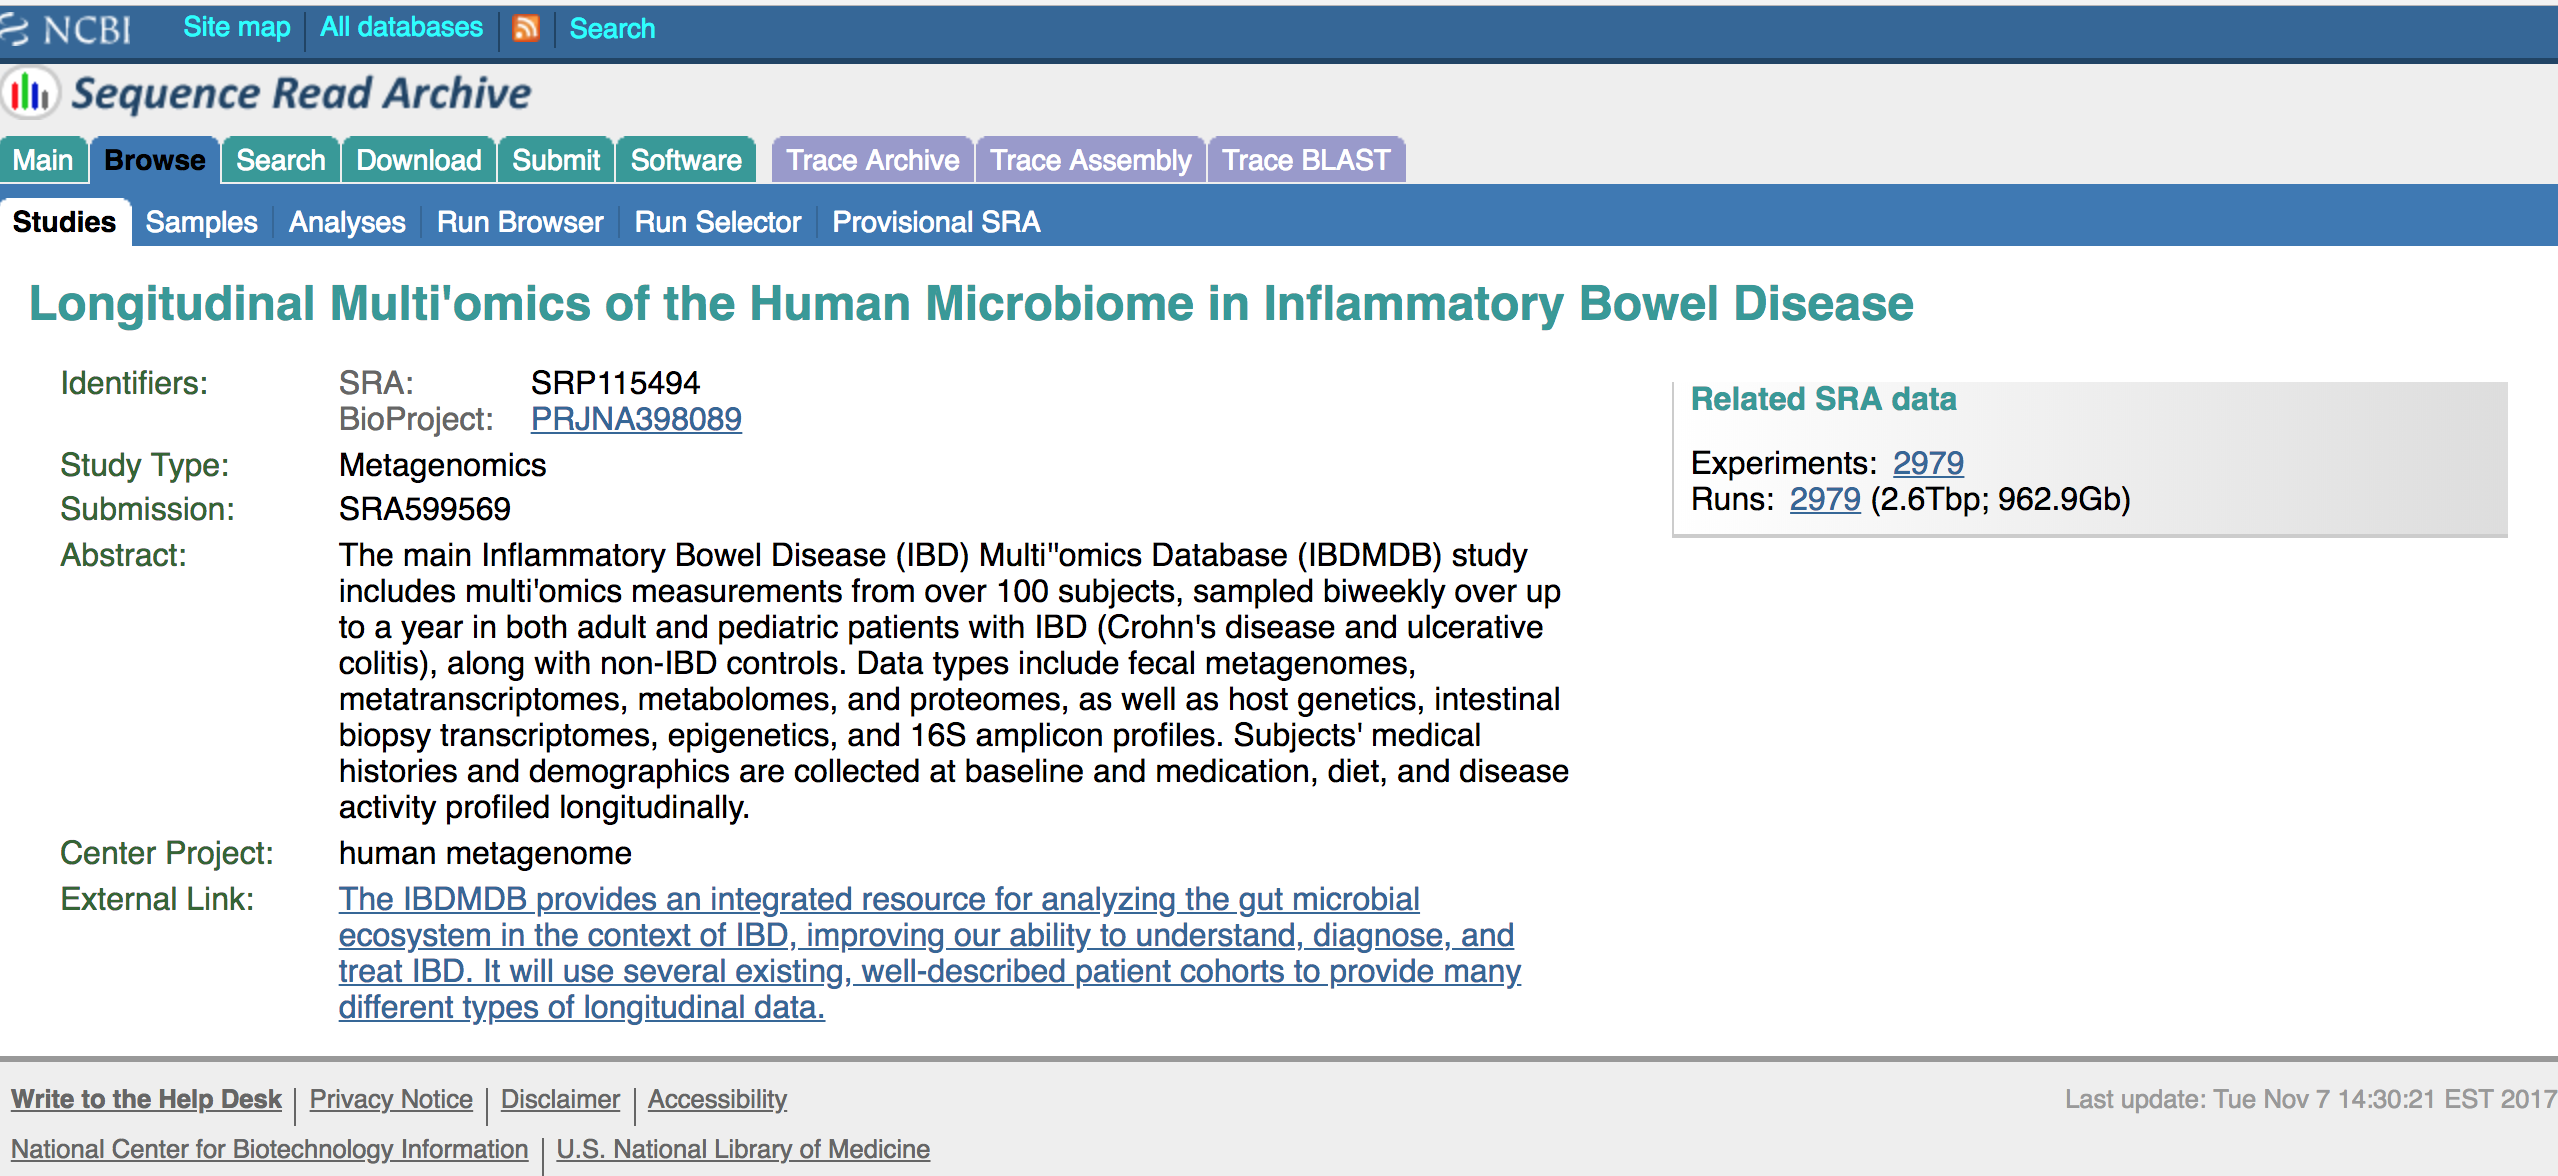
\includegraphics[height=8.75cm, width=16cm]{ncbi-sra-study-page}
    \caption{The "SRA Study" webpage.}
    \label{fig:ncbi-sra-study-page}
    \end{maxipage}
\end{figure}
%

The dataset is reproduced in Figure \ref{fig:ncbi-sra-runs-page} and can be found by clicking on "Runs" under "Related SRA data" on the right side of the SRA Study webpage, or by going to \url{https://trace.ncbi.nlm.nih.gov/Traces/study/?acc=SRP115494#} .

%
\begin{figure}[hbtp]
    \begin{maxipage}
    %\begin{center}
    \centering
    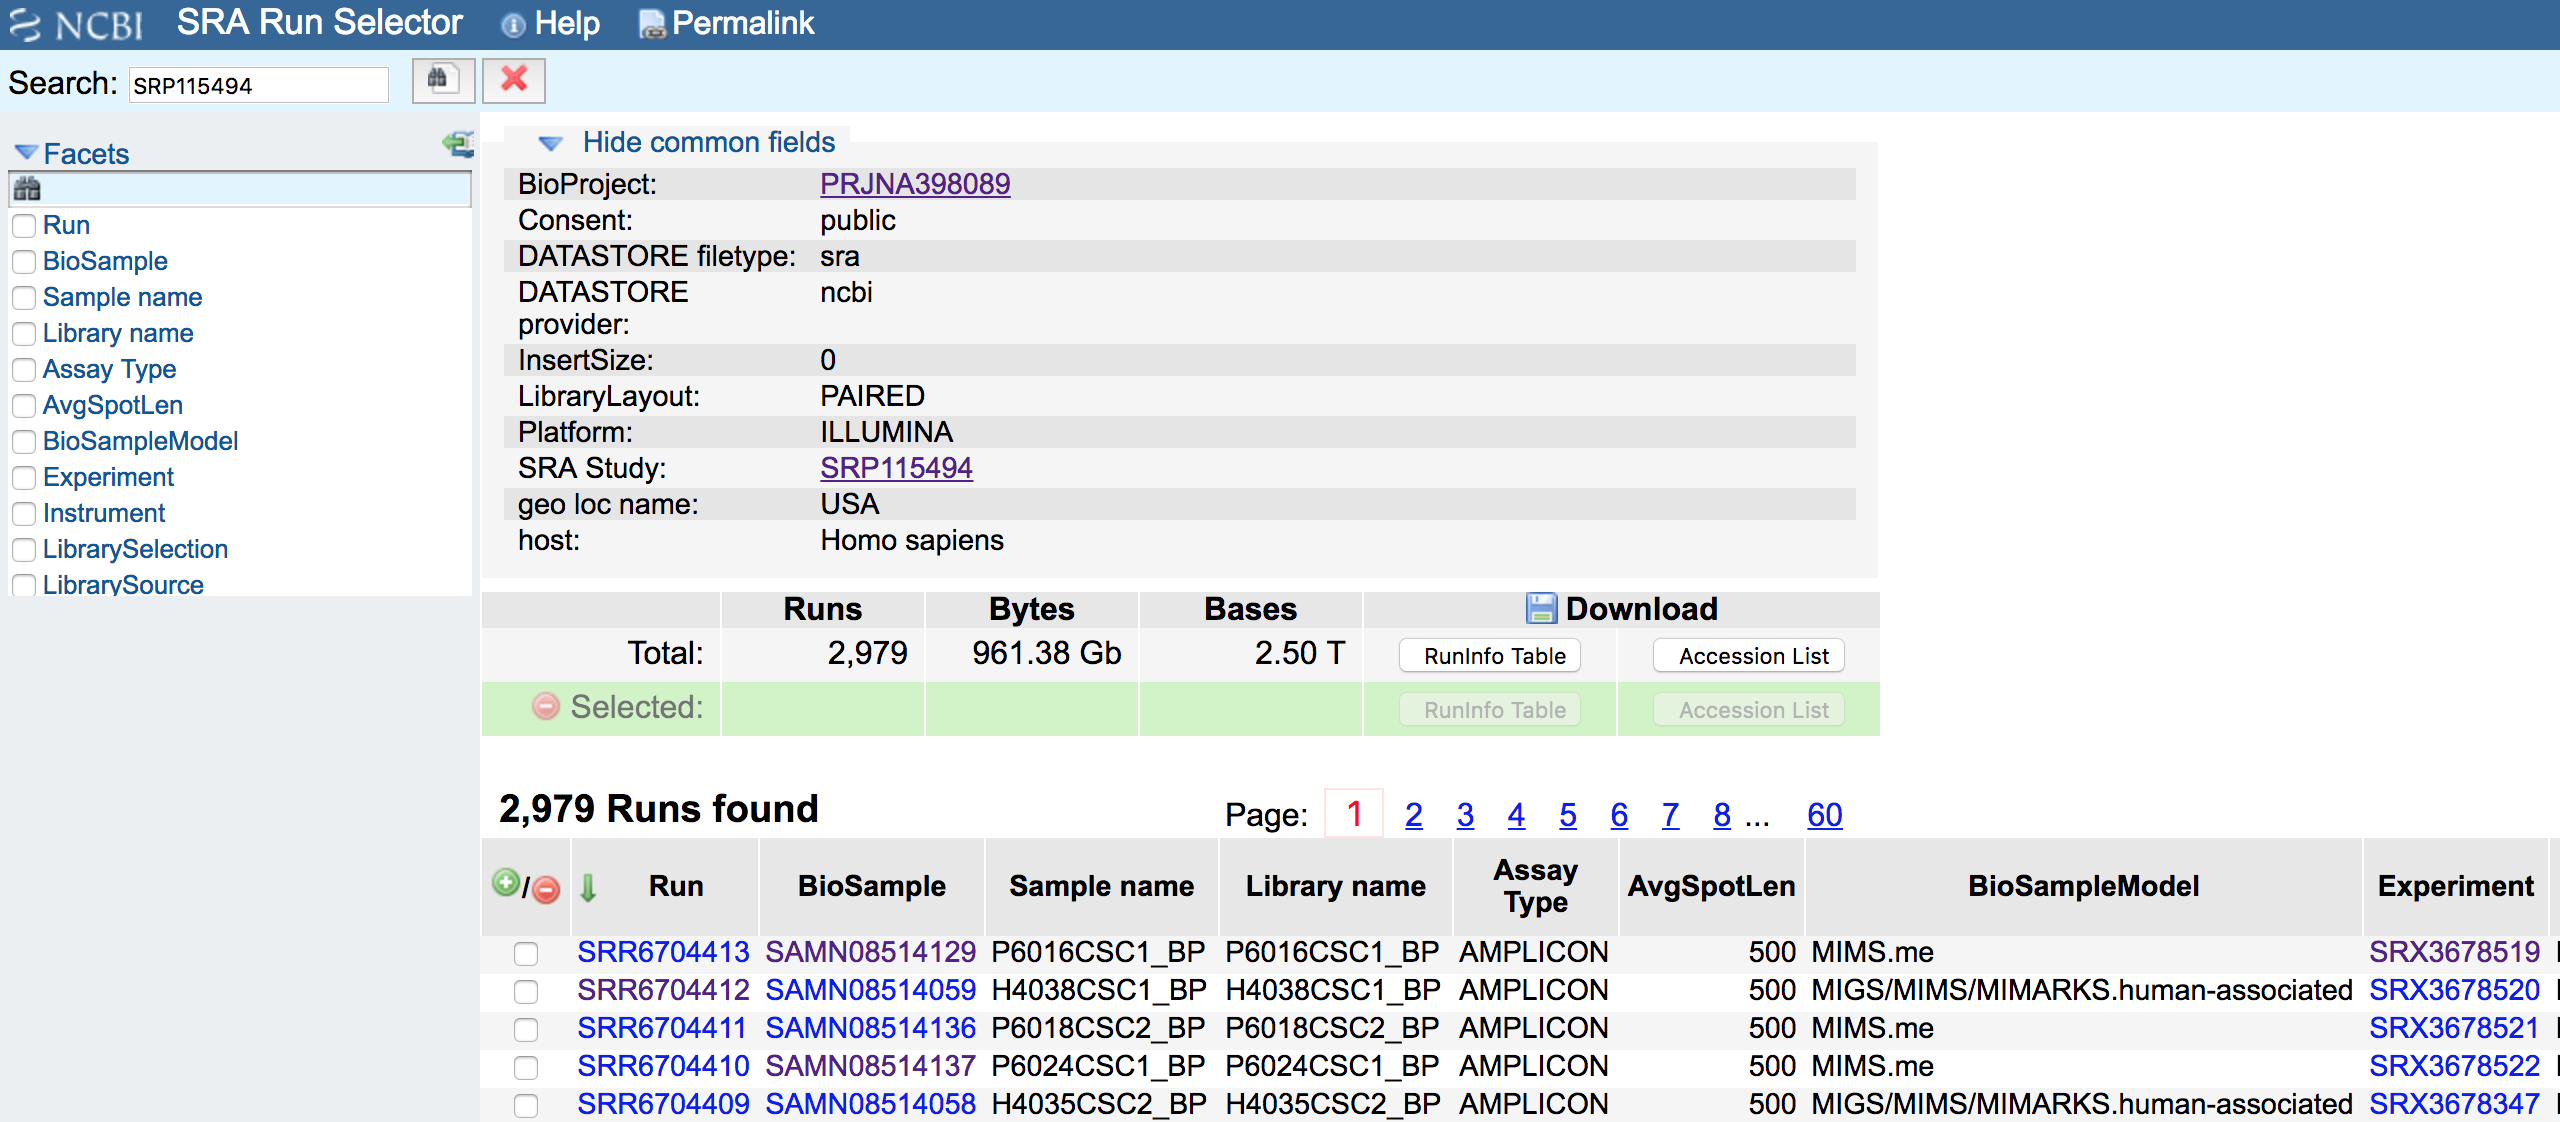
\includegraphics[height=8.5cm, width=16cm]{ncbi-sra-runs-page}
    \caption{The sequencing data collected by the \textit{Longitudinal Multi'omics of the Human Microbiome in Inflammatory Bowel Disease} study. (Note: the table's columns extend beyond the right side of the page because there are 36 metadata categories.)}
    \label{fig:ncbi-sra-runs-page}
    %\end{center}
    \end{maxipage}
\end{figure}
%
    
To learn more about how to use these pages to find information about the study and its methods, please refer to Chapter \ref{chap:find-tools}. 
    
    %
    \section{Download Dataset}
    \todo[inline]{*****Show the user what the result of the commands are. Right now we show the commands, but not the results. e.g., when we run a command to get a list of accession numbers, follow it up by typing the command that just prints the list of numbers in the terminal. Then the user can see what their results should look like if they did everything correctly. }
    
    \subsection*{1) Choose sample criteria}
        \begin{enumerate}
            \item First, we must decide what criteria we will use to choose our experimental samples. 
            \marginlabel{Note: The dataset has a metadata category called "BioSample." This is not to be confused with the generic term "samples", which in this case are equivalent to one run (i.e., one row) of the data table.}
            \newline
            Remember: our research question investigates the effects of age on the gut microbiomes of inflammatory bowel disease patients. Looking at the study abstract from Figure \ref{fig:ncbi-sra-study-page}, we can see that the researchers investigated two types of IBD: Crohn's disease and ulcerative colitis. So one of the metadata categories from the dataset (i.e., the columns from the dataset in Figure \ref{fig:ncbi-sra-runs-page}) that we will use to select our samples is the "host\_disease" category. We will also select our samples based on the "host\_age" metadata.
            
            \item Now we want to select our samples based on these categories. 
            
            Download the RunInfo Table file found on the study's sample page and put it in the project folder you set up in Chapter \ref{software}. The RunInfo table is the browser's sample table in a .txt file format.
            \missingfigure{highlight where to click to download the runinfo table}
            
            \item Open the command line interface for your machine's operating system. On a mac, this is the Terminal application. 
            
            \item Navigate to your project's folder and then confirm that you are in the right location by using the the following commands at the command prompt:
            
                \begin{lstlisting} [language=Python]
$ cd <path\_to\_your\_project>
$ pwd
                \end{lstlisting}
                        
            \item Activate the Python interpreter by typing the following into the command prompt:
                \begin{lstlisting} [language=Python]
$ python3
                \end{lstlisting}
            
            \item Import BioPype to the current Python environment:
                \begin{lstlisting} [language=Python]
>>> import BioPype
                \end{lstlisting}
                
                    \begin{itemize}
                    \item \attention{If not done already, stop and follow the instructions in Chapter \ref{chap:software} to configure the BioPype working directory and the SRA Toolkit Workspace Location.}
                    \end{itemize}
                
            \item Import \verb|BioPype.cmds.runtable| to gain access to the \verb|RunTable| class:
            \todo[inline]{Either shorten this margin-label, or put it in a footnote.}
            \marginlabel{Using "as" in an import statement lets you reference the full name of the imported package by some shorter name. It is generally considered better practice to \textbf{not} import packages "as" some other name, because it makes the code less explicit (which goes against the purpose of Python), but we do it in this manual for the sake of space.}
                \begin{lstlisting} [basicstyle=\small, language=Python]
>>> import BioPype.cmds.runtable as runtable
                \end{lstlisting}
                
            \item Create a \verb|RunTable| object called "my\_table" out of the RunInfo Table .txt file:
            \todo[inline]{Give a specific name to the RunInfo Table file. People might get confused if they needs to fill in the name of the file themselves.}
            \begin{lstlisting} [basicstyle=\footnotesize, language=Python]
>>> my_table = runtable.RunTable('runinfotable_filename.txt')
            \end{lstlisting}
            
            
                \begin{itemize}
                \item With the \verb|my_table| object created, you can remind yourself what the metadata categories are by using the following command:
                \end{itemize}
                \begin{lstlisting} [basicstyle=\footnotesize, language=Python]
>>> my_table.column_names
['Assay_Type', 'AvgSpotLen', 'BioSample', 'BioSampleModel', 
 'Experiment', 'Instrument', 'LibrarySelection', 'LibrarySource', 
 'Library_Name', 'LoadDate', 'MBases', 'MBytes', 'Organism', 
 'ReleaseDate', 'Run', 'SRA_Sample', 'Sample_Name', 
 'collection_date', 'env_biome', 'env_feature', 'env_material', 
 'host_age', 'host_disease', 'host_sex', 'host_subject_id', 
 'lat_lon', 'BioProject', 'Consent', 'DATASTORE_filetype', 
 'DATASTORE_provider', 'InsertSize', 'LibraryLayout', 'Platform', 
 'SRA_Study', 'geo_loc_name', 'host']
                \end{lstlisting}
                
                
            \item We want to first group the samples based on the patients' disease...
            \begin{lstlisting} [basicstyle=\scriptsize, language=Python]
>>>uc_samples=my_table.filter_data("host_disease", '==', 'ulcerative colitis')
>>>cd_samples=my_table.filter_data("host_disease", '==', "Crohn''s disease")
            \end{lstlisting}
                \begin{itemize}
                \item \attention{Note} that the "Crohn's disease" string within the parentheses in the second line of code has two single-quotes/apostrophes between the "n" and the "s" of "Crohn's". This is because the value we input must exactly match the value that the original study's researchers input for the \verb|host_disease| category, and (for whatever reason) they entered the value for Crohn's disease as:   \verb|"Crohn''s disease"|
                
                This is an example of why it's important to check the metadata carefully before you begin the analysis. If the argument does not exactly match the value of the metadata category, it won't select the sample. 
                \end{itemize}
            
                
            \item ... then we want to group them based on age:
            \begin{lstlisting} [basicstyle=\small, language=Python]
>>>uc_young = uc_samples.filter_data("host_age", '<=', 21)
>>>uc_old = uc_samples.filter_data("host_age", '>=', 60)
>>>cd_young = cd_samples.filter_data("host_age", '<=', 21)
>>>cd_old = cd_samples.filter_data("host_age", '>=', 60)
            \end{lstlisting}
                \begin{itemize}
                \item \attention{Note} that the third argument passed to the \verb|filter_data()| method is \textbf{not} a string like the previous two arguments. It is simply an integer (no quotation marks around it).
                \end{itemize}
                
                
            \item Now that we have groups of samples selected, we want to get a list of SRA accession numbers for each group. The accession numbers are what we will use to specify the files we want to download from the SRA database. 
            \begin{lstlisting} [basicstyle=\small, language=Python]
>>>uc_young_nums = uc_young.get_accession_numbers()
>>>uc_old_nums = uc_old.get_accession_numbers()
>>>cd_young_nums = cd_young.get_accession_numbers()
>>>cd_old_nums = cd_old.get_accession_numbers()
            \end{lstlisting}
            
            
            \item \seealso{To learn more about .sra file format, see Appendix \ref{app:sra-format}.}
            We can now use the lists of accession numbers to download .sra files from the SRA database. However, these are large files that can \textit{easily} take up hundreds of gigabytes of memory. They also take time to download (times will vary based on network speed). To account for hardware limitations that would severely bottleneck the analysis at file-handling steps like these, we will randomly select a subset of only 3 accession numbers from each list we created in the previous step. The analysis will go much faster if we analyze fewer samples, so these subsets are what we will analyze going forward.
            \seealso{The "random\_sample\_ subset()" method is preceded by "RunTable." in this case because it is a "@staticmethod". To learn more, see Appendix \ref{app:static-method}.}
            \begin{lstlisting} [basicstyle=\footnotesize, language=Python]
# Shorten the name for the runtable module to save space in the manual:
>>>import BioPype.cmds.runtable as rt

>>>rs_uc_young = rt.RunTable.random_sample_subset(uc_young_nums, n=3)
>>>rs_uc_old = rt.RunTable.random_sample_subset(uc_old_nums, n=3)
>>>rs_cd_young = rt.RunTable.random_sample_subset(cd_young_nums, n=3)
>>>rs_cd_old = rt.RunTable.random_sample_subset(cd_old_nums, n=3)
            \end{lstlisting}
            
            
            \item Now we need to download the .sra files linked to these accession numbers and get them into .fastq format. First, we'll need to import the necessary functions:
            \begin{lstlisting} [basicstyle=\small, language=Python]
>>>from BioPype.cmds.downloadsra import download_sra,
>>>from BioPype.cmds.downloadsra import convert_sra_to_fastq
            \end{lstlisting}
            
            
            \item Use the \verb|download_sra()| function to download the .sra files into named folders:
            \begin{lstlisting} [language=Python]
>>>download_sra(rs_uc_young, 'uc_young')
>>>download_sra(rs_uc_old, 'uc_old')
>>>download_sra(rs_cd_young, 'cd_young')
>>>download_sra(rs_cd_old, 'cd_old')
            \end{lstlisting}
                \begin{itemize}
                \item \attention{The .sra files will not be downloaded to the correct location if the SRA Toolkit Workspace Location has not been properly configured (see Chapter \ref{chap:software} for details).}
                \end{itemize}
            
            
            \item \seealso{To learn more about .fastq format, see Appendix \ref{app:fastq-format}.} 
            Use the \verb|convert_sra_to_fastq()| function to convert the .sra files to .fastq format.
            
            \seealso{To learn more about what threads are, and how many you should use, see Appendix \ref{app:threads}.}
            \begin{lstlisting} [language=Python]
>>>convert_sra_to_fastq(threads=4)
            \end{lstlisting}
                \begin{itemize}
                \item \attention{BioPype will not know where to look for the downloaded .sra files if the SRA Toolkit Workspace Location has not been properly configured (see Chapter \ref{chap:software} for details).}
                \item The more threads your computer can divide this process between, the better (it's more complicated than that, but for now let's go with it). The question is: how many threads is your computer capable of using? For that, you'll have to do some Googling. You can find the resources I used to figure out how many threads my MacBook Pro can run (4) in Appendix \ref{app:threads-resources}. To simplify: my computer has 1 CPU, the CPU has 2 cores, and each core can run 2 threads. 1 x 2 x 2 = 4 threads.
                \end{itemize}            
                                    
        \end{enumerate}
        
        %
        \subsection{Creating the code}
        
        %
    
    
    \section{Perform Quality Control on Dataset}

